\section{Sicherungsschicht}

\paragraph{Terminologie}
\begin{itemize}
  \item \textbf{Knoten}: Endsysteme + Router
  \item \textbf{Links}: Übertragungsabschnitt zwischen benachbarten Knoten
  \item \textbf{Rahmen}: Pakete auf Schicht 2 (IP-Datagramme eingekapselt)
  \item \textbf{Aufgabe}: Übertragung von Datagrammen zw Nachbarknoten über Link
\end{itemize}

\paragraph{Aufgaben}
\begin{itemize}
  \item \textbf{Strukturierung} des Datenstroms (\emph{framing}) \\* \( \leadsto \) Datagramm in Rahmen einkapseln hinzufügen
  \item \textbf{Medienzugangskontrolle} bei geteilten Medien
  \item \textbf{Adressierung} mittels MAC-Adressen
  \item Je nach angebotenem Dienst \emph{Fehlererkennung/-behebung} bzw. \emph{Flusskontrolle}
  \item \textbf{(Semi-) Broadcast}: Alle Stationen sehen alle Rahmen (zB WLAN = semi-broadcast)
  \item \textbf{Punkt-zu-Punkt-Link}: Zwei Stationen sind über dedizierten Link verbunden (zB switch-basiertes Ethernet)
  \begin{itemize}
    \item \emph{Simplex}: Übertragung in eine Richtung
    \item \emph{Halbduplex}: Übertragung in beide Richtungen, nicht zeitgleich
    \item \emph{(Voll-) Duplex}: Übertragung in beide Richtungen, zeitgleich
  \end{itemize}
\end{itemize}

\paragraph{Sicherungsschicht --- Implementierung}
Sicherungsschicht ist in jedem Knoten (Endsystem, Router, Switch) implementiert (auf Netzadapter oder auf Chip), an Systembus angeschlossen (Kombination von Hardware, Software und Firmware)

\paragraph{Sicherungsschicht --- Fehlererkennung}
\begin{itemize}
  \item \textbf{Wie Schicht 4}: Erkennung/Behebung von Bit- und Paketfehlern
  \item \textbf{Unterschied Schicht 4}:
  \begin{itemize}
    \item zu sendende/empfangende Bitfolge wird bitseriell betrachtet
    \item Internetprüfsumme basiert auf Wörtern, die bereits im Speicher stehen
  \end{itemize}
  \item Rahmen erhält Sicherungssequenz \emph{frame check sequence} (FCS, üblicherweise als Anhang am Rahmenende)
\end{itemize}

\paragraph{Fehlererkennung --- cyclic redundancy check (CRC)}
\begin{itemize}
	\item Jede zyklische Verschiebung eines Codeworts führt wieder zu einem Codewort
  \item \textbf{Code \( \to \) Polynom}: \code{0101} \( \to 0x^3+1x^2+0x^1+1x^0 = x^2+1 \)
  \item \textbf{Generatorpolynom}: von \( G(x) \) generierte Code ist \\* \( C \coloneqq \{ v(x) \mid \text{deg}(v(x)) < n \wedge G(x) \text{ teilt } v(x) \} \)
  \item \textbf{Prinzip}:
  \begin{itemize}
    \item gleiches Polynom \( G(x) \) für Sender und Empfänger
    \item \emph{Sender}:
    \begin{itemize}
      \item  \( m \) Bit Rahmen \( \to M(x) \) (Polynom/Codewort)
      \item hängt \( r = \text{deg}(G(x)) \) Nullen an Daten (\( \to x^r \cdot M(x) \))
      \item berechnet Rest von \( M(x)/G(x) \)
      \item hängt Rest an ursprüngliche Daten (statt der Nullen von oben)
    \end{itemize}
    \item \emph{Empfänger}: Dividiert durch \( G(x) \)
    \begin{itemize}
      \item Ergebnis \( 0 \): keine Fehler erkannt
      \item Ergebnis \( \neq 0 \): Fehler!
    \end{itemize}
  \end{itemize}
\end{itemize}

\paragraph{CRC --- Hardwareimplementierung}
\begin{itemize}
  \item Rückgekoppelte Schieberegister \( \to \) CRC bei Durchschieben berechnet
  \item \textbf{Prinzip}:
  \begin{itemize}
    \item Bitweises Empfangen der Daten, durchlaufen Schieberegister
    \item Rückkopplung durch \code{XOR}-Gatter an 1-Stellen des Gens (ohne höchstes Bit)
    \item Nach Durchlaufen von Codewort + angehängte 0en Prüfsumme im Register
  \end{itemize}
\end{itemize}
\begin{figure}[H]\centering\label{Schieberegister}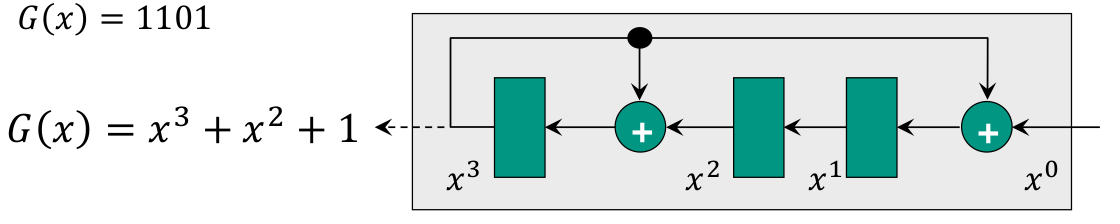
\includegraphics[width=0.33\textwidth]{Schieberegister}\end{figure}

\paragraph{Multiplexing --- Medienzugriff}
\begin{itemize}
  \item \textbf{Problem}: Link von mehreren Knoten parallel benutzt
  \item \textbf{Varianten}:
  \begin{itemize}
    \item feste Mediumszuteilung (eine Dimension, Punkt-zu-Punkt-Verbindungen)
    \item konkurrierende Nutzung \( \to \) Zugriffsorganisation notwendig
  \end{itemize}
  \item \textbf{Dimensionen}: Raum \( r \), Zeit \( t \), Frequenz \( f \), Code \( c \)
  \item \textbf{Wichtig}: Schutzabstände erforderlich
\end{itemize}

\paragraph{Multiplexing --- Raum}
\begin{itemize}
  \item Raumeinteilung in Sektoren (zB gerichtete Antennen)
  \item \textbf{Kupfermultiplex}: Zuordnung dedizierter Leitungen
  \item \textbf{Einsatz}: Mobilfunkzellen
  \item Space Division Multiple Access (SDMA)
\end{itemize}

\paragraph{Multiplexing --- Frequenz}
\begin{itemize}
  \item \textbf{Prinzip}: verfügbare Bandbreite wird in Frequenzabschnitte unterteilt
  \item \textbf{Vorteile}:
  \begin{itemize}
    \item keine dynamische Koordination nötig
    \item auch für analoge Signale möglich
  \end{itemize}
  \item \textbf{Nachteile}:
  \begin{itemize}
    \item Bandbreitenverschwendung bei ungleichmäßiger Auslastung
    \item unflexibel
  \end{itemize}
  \item \textbf{Einsatz}: DSL
\end{itemize}

\paragraph{Multiplexing --- Zeit}
\begin{itemize}
  \item \textbf{Prinzip}: Kanal belegt ganzen Frequenzraum für festgelegte Zeit
  \item \textbf{Vorteile}:
  \begin{itemize}
    \item nur ein Träger gleichzeitig auf Medium
    \item auch bei großer Teilnehmerzahl hoher Durchsatz
  \end{itemize}
  \item \textbf{Nachteil}: genaue Synchronisation nötig
  \item \textbf{Einsatz}: Ethernet, WLAN
  \item \textbf{Hinweis}: Standard-Multiplexverfahren im Folgenden
\end{itemize}

\paragraph{Multiplexing --- Code}
\begin{itemize}
  \item \textbf{Prinzip}: alle Stationen zur gleichen Zeit auf gleicher Frequenz
  \begin{itemize}
    \item \emph{Sender}: verknüpft Signal mit eindeutiger Pseudozufallszahl
    \item \emph{Empfänger}: kann mithilfe bekannter Pseudozufallszahlfolge + Korrelationsfunktion Originalsignal wiederherstellen
  \end{itemize}
  \item \textbf{Vorteile}:
  \begin{itemize}
    \item keine Frequenzplanung erforderlich
    \item großer Coderaum im Vergleich zu Frequenzraum
    \item Vorwärtskorrektur + Verschlüsselung leicht integrierbar
  \end{itemize}
  \item \textbf{Nachteile}:
  \begin{itemize}
    \item höhere Komplexität wegen Signalregenerierung
    \item alle Signale müssen bei Empfänger gleich stark ankommen
  \end{itemize}
  \item \textbf{Einsatz}: UMTS
\end{itemize}

\paragraph{Zeitmultiplex --- Zufallsstrategien}
\begin{itemize}
  \item \textbf{Aloha}: zufällige, unabh, seltenes Senden; gleichzeitiges Senden = Kollision
  \item \textbf{Slotted Aloha}: Verbesserung von Aloha, Erfordert Knotensynchronisation
    \begin{figure}[H]\centering\label{SlottedAloha}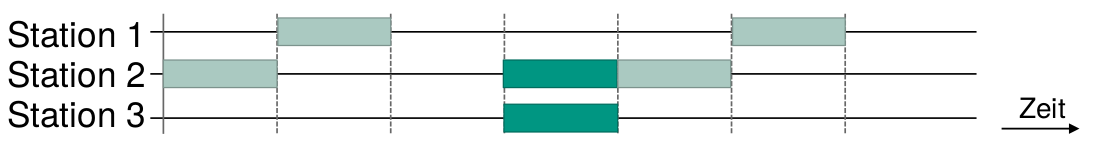
\includegraphics[width=0.33\textwidth]{SlottedAloha}\end{figure}
  \item \textbf{CSMA} (\emph{carrier sense multiple access}):
  \begin{itemize}
    \item \emph{Prinzip}: Andere nicht unterbrechen während sie reden
    \item \emph{listen before talk}: System prüft vor Senden, ob Medium frei ist
    \item \emph{Medium belegt}: später erneut versuchen
    \item \emph{Medium frei}: Senden
    \item \emph{Kollisionen}, wenn mehrere Systeme gleichzeitig zu Senden beginnen
  \end{itemize}
  \item \textbf{CSMA/CD} (\emph{CSMA with collision detection})
  \begin{itemize}
    \item \emph{listen while talk}: Kollisionserkennung durch Abhören während des Sendens
    \item \emph{Kollision}: Sendungsabbruch, später neu versuchen
  \end{itemize}
\end{itemize}

\paragraph{Zeitmultiplex --- Umsetzung Ethernet}
\begin{itemize}
  \item \textbf{Kollision}:
  \begin{enumerate}
    \item Sendungsabbruch
    \item Sender sendet \emph{Jamming-Signal}
    \item \emph{Backoff-Algorithmus} regelt Sendungswiederholung
  \end{enumerate}
  \item \textbf{Vorraussetzungen}:
  \begin{itemize}
    \item Senden der Rahmen darf nach Signallaufzeit durch Medium und zurück noch nicht fertig sein
    \item Mindestlänge für Rahmen (abhängig von Netzausdehnung + Ausbreitungsgeschwindigkeit) erforderlich
    \item zu kleiner Rahmen: Auffüllen auf Mindestlänge (\emph{padding})
  \end{itemize}
\end{itemize}

\paragraph{Kollisionsfreier Zugriff --- Prinzip}
\begin{itemize}
  \item \textbf{Polling}: Kontrolle durch zentralen Knoten
  \begin{itemize}
    \item Senderecht sequentiell zugewiesen
    \item \emph{Nachteil}: koordinierender Knoten nötig, kann ausfallen
    \item \emph{Einsatz}: Bluetooth
  \end{itemize}
  \item \textbf{Token Passing}: Senderechtsweitergabe von Knoten zu Knoten
  \begin{itemize}
    \item \emph{Nachteil}: Knoten können ausfallen \( \to \) Zugriff blockiert
    \item \emph{Einsatz}: Token Ring
  \end{itemize}
\end{itemize}

\paragraph{Kollisionsfreier Zugriff --- Token Ring}
\begin{itemize}
  \item \textbf{Prinzip}:
  \begin{itemize}
    \item Systeme physikalisch Punkt-zu-Punkt-verbunden zu Ring
    \item Jedes System hat \emph{Vorgänger} und \emph{Nachfolger}
    \item Senderechtszuteilung durch zirkulierendes Token
    \item Sendendes System nimmt Daten auch wieder vom Ring
  \end{itemize}
  \item Monitor: Endsystem zur Überwachung des Rings, Tokenmanagement (komplex!)
  \item Strukturierte Verkabelung von Gebäuden, Viele Endsysteme möglich
\end{itemize}

\paragraph{Kollisionsfreier Zugriff --- Token Bus}
\begin{itemize}
  \item \textbf{Prinzip}:
  \begin{itemize}
    \item Verbindet Vorteile von Ethernet und Token Ring
    \item Busverkabelung wie bei Ethernet (robust: Ausfall eines Endsystem für Netz egal)
    \item \emph{Garantierte Antwortzeiten} durch zirkulierendes Token
  \end{itemize}
  \item \textbf{Aufbau}:
  \begin{itemize}
    \item Alle Stationen physikalisch durch Bus verbunden
    \item Bildung eines \emph{logischen Rings}
  \end{itemize}
\end{itemize}
\begin{figure}[H]\centering\label{TokenBus}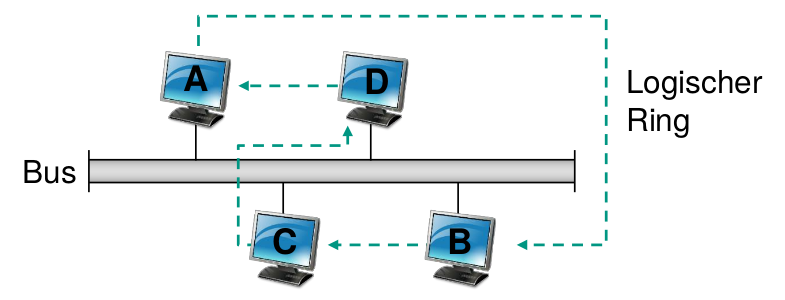
\includegraphics[width=.5\linewidth]{TokenBus}\end{figure}

\paragraph{Lokale Netze --- MAC-Adressen}
\begin{itemize}
  \item Theoretisch weltweit eindeutig
  \item Jeder Netzadapter muss in einem lokalen Netz eindeutige MAC-Adresse haben
  \item \textbf{Funktion}: lokal genutzt, um Rahmen von Interface zu benachbartem, physikalisch verbundenem Interface zu übertragen
  \item \textbf{Format}:
  \begin{itemize}
    \item 48 Bit (24 Bit von IEEE an Hersteller zugewiesen, 24 Bit durchnummeriert)
    \item stehen im NIC-ROM, können aber auch per Software gesetzt werden
    \item Darstellung meist hexadezimal (zB \code{24-2F-EA-76-CC-28})
    \item Broadcast: \code{FF-FF-FF-FF-FF-FF}
  \end{itemize}
\end{itemize}

\paragraph{Lokale Netze --- address resolution protocol (ARP)}
\begin{itemize}
  \item \textbf{Problem}: Welche MAC-Adresse hat nächstes System im eigenen Subnetz?
  \item \textbf{Aufgabe}: MAC-Adresse zu bekannter IP-Adresse ermitteln
  \item \textbf{Prinzip}: dynamisch Adresszuordnungen lernen
  \item \textbf{ARP-Cache}: kleine Tabelle auf jedem System, Einträge bei Bedarf gelernt; Eintrag IP + MAC + maximale Lebenszeit (typisch 20 Minuten) 
\end{itemize}

\paragraph{ARP --- Adressauflösung}
\begin{itemize}
  \item \textbf{Szenario 1}: \( A \) sendet Datagramm an \( B \) in selbem Subnetz
  \begin{itemize}
    \item \emph{Fall 1}: ARP-Cache von \( A \) hat Eintrag für \( B \) \( \to \) Paket verschicken, Timeout neu setzen
    \item \emph{Fall 2}: ARP-Cache von \( A \) hat Eintrag für \( B \) \emph{nicht} \( \to \) Broadcast \emph{ARP-Request} mit IP von \( B \), Jeder Knoten liest ARP-Request (ARP-Reply falls eigene IP), \( A \) trägt Infos in ARP-Cache ein
  \end{itemize}
  \item \textbf{Szenario 2}: \( A \) sendet Datagramm an \( B \) in anderem Subnetz
  \begin{enumerate}
    \item \( A \) sendet ARP-Request für Router \( R \)
    \item \( A \) sendet Datagramm an IP von \( B \) und MAC von \( R \)
    \item Router empfängt Datagramm, setzt Ziel-MAC auf \( B \), Sender-MAC auf \( R \)
    \item Router leitet Datagramm weiter
  \end{enumerate}
\end{itemize}

\paragraph{Lokale Netze --- Ethernet (IEEE 802.3)}
\begin{itemize}
  \item \textbf{Medienzuteilung}:
  \begin{itemize}
    \item zeitmultiplex, variabel, zufälliger Zugriff, CSMA/CD
    \item Kanal wird logisch in Zeitschlitze fester Länge aufgeteilt
    \item Dauer = minimale Rahmenlänge, Kollisionserkennung vor Zeitschlitz-Ende
    \item Exponentieller Backoff: Warte nach Kollision \( i \) zufällig [0, \( 2^i-1 \)] Zeitschl
  \end{itemize}
  \item \textbf{Netztopologie}: Ursprünglich Bus-, heute Sterntopologie (Switches statt Repeatern)
  \item \textbf{Varianten}: [Datenrate][Baseband/Broadband][Medium] (z.B. 10Base5)
   \item Ethernet-Rahmen (immer gleich)
   \begin{figure}[H]\centering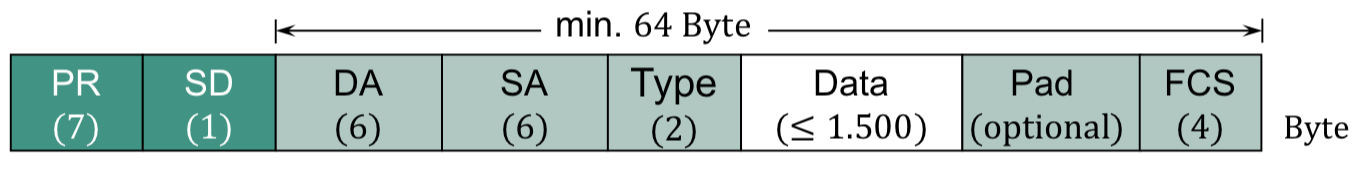
\includegraphics[width=.8\linewidth]{Ethernet}\end{figure}
   Präambel, Start of Frame Delimiter, Destination Address, Source Address, Type/Length, Data, Padding, Frame Check Sequence
\end{itemize}

\paragraph{Ethernet --- Switches}
\begin{itemize}
  \item \textbf{Prinzip}: Schicht-2-Netzkopplung (innerhalb \emph{eines} IP-Subnetzes)
  \begin{itemize}
    \item Leitet Rahmen zwischen Interfaces weiter und puffert sie zwischen
    \item Trennung von Inter- und Intranetz-Verkehr \( \to \) Erhöhung Netzkapazität
    \item Switches nicht sichtbar für Endsysteme
  \end{itemize}
  \item \textbf{Ziel}: Selbstorganisierte Netzkonfiguration mit Switches
  \item \textbf{Aufgaben}:
  \begin{itemize}
    \item Schleifenfreie Netztopologie (\emph{spanning tree} Algorithmus)
    \item Wege zwischen Endsystemen (selbstlernend; Ziel unbekannt: Fluten)
  \end{itemize}
\end{itemize}

\paragraph{Ethernet --- Kollisionsdomänen}
Netzbereich, der von Kollision betroffen ist (gemeinsames Broadcastmedium)
\begin{figure}[H]\centering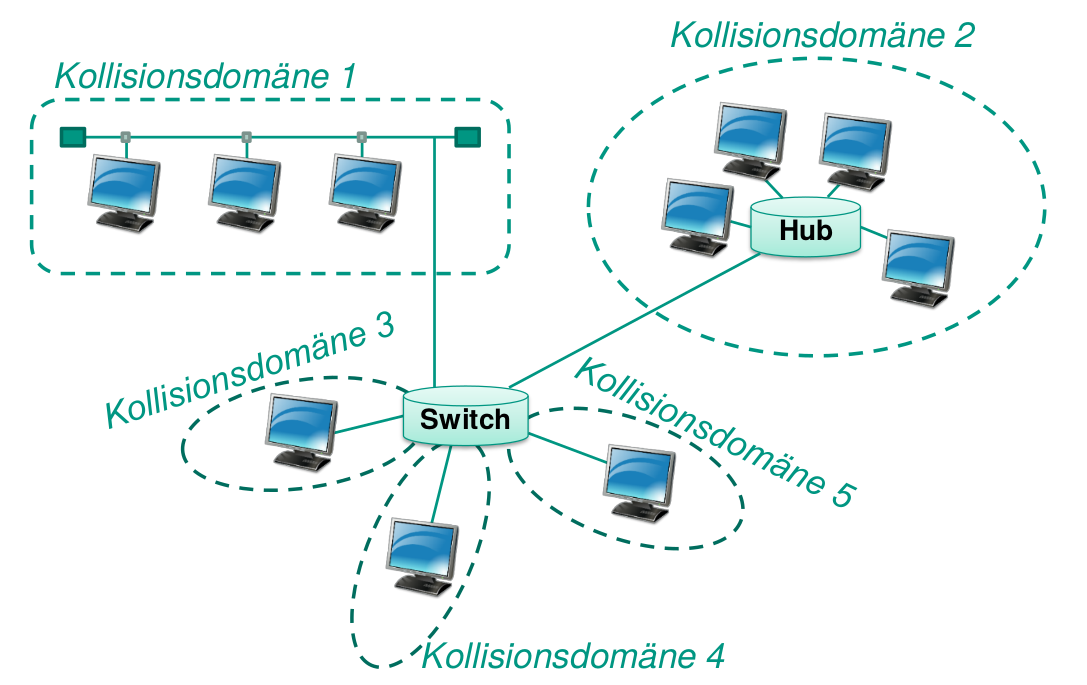
\includegraphics[width=0.33\textwidth]{Kollisionsdomaenen}\end{figure}

\paragraph{virtual local area network (VLAN)}
\begin{itemize}
  \item \textbf{Idee}: Logische Trennung von Datenverkehr auf Ethernet-Ebene \\* \( \leadsto \) virtuelle Leitung
  \item \textbf{Sicherheit}: Trennung in logische Medien \( \to \) gezielte Systemgruppierung + bessere Netzstruktur-Kontrolle
  \item \textbf{Flexibilität}:
  \begin{itemize}
    \item Einfache Reorganisation der logischen Medien möglich
    \item keine Änderungen an physikalischem Medium (Neuverkabelung) nötig
  \end{itemize}
  \item \textbf{Performance}: Broadcast-Last eines Netzes sinkt, wenn physikalisches Medium in mehrere logische aufgeteilt wird
\end{itemize}

\paragraph{VLAN --- Interface-basiert}
\begin{itemize}
	\item Ein einziger physikalischer Switch arbeitet als mehrere virtuelle Switches
	\item Jeweils mehrere Interfaces werden zu einem virtuellen Switch gruppiert
  \item \textbf{Verkehrsisolation}: Rahmen von einem Interface können nur Interfaces in der gleichen Gruppe erreichen \( \leadsto \) Sicherheit, Performance
  \item \textbf{Flexible Zuweisung}: Interfaces dynamisch anderen VLANs zuordnen
  \item \textbf{Weiterleitung} zwischen VLANs über Routing
  \item \textbf{Trunks}: Transport von Rahmen zwischen multi-switch-VLANs
  \begin{itemize}
    \item \emph{VLAN-ID}: Jedes VLAN erhält Kennzeichner
    \item Ethernet-Frames werden mit VLAN-ID getaggt
    \item Switches entfernen Tagging vor Auslieferung an Endsystem
  \end{itemize}
\end{itemize}